
\section{Phần cứng thực nghiệm \label{section_overview_propsed_method}}
\subsection{Cảm biến \label{section_overview_propsed_method}}

Trong quá trình ngủ, các chuyển động thân thể chủ yếu là chuyển động 
chậm, với biên độ nhỏ và không mang tính đột ngột. 
Các chuyển động thân thể chủ yếu mang tính chậm và thường xảy ra 
trong giai đoạn ngủ không chuyển động mắt nhanh (NREM), 
khi cơ thể có khả năng tự do thay đổi tư thế. Ngược lại, 
trong giai đoạn ngủ REM, hiện tượng ức chế trương lực cơ khiến 
cơ thể gần như bất động.
Do đó, việc ghi 
nhận chính xác các thay đổi tư thế ngủ đòi hỏi cảm biến có độ nhạy cao, 
khả năng phân giải tốt và ổn định với nhiễu nền thấp. Như đã trình bày 
trong Chương I, các cảm biến gia tốc MEMS sử dụng nguyên lý điện dung 
hiện đang được ứng dụng rộng rãi trong giám sát tư thế và chuyển động 
khi ngủ nhờ vào đặc điểm nổi bật là kích thước nhỏ gọn, tiêu thụ năng 
lượng thấp, tần số lấy mẫu phù hợp và đặc biệt là độ nhạy cao với 
chuyển động cường độ thấp.

Trong nghiên cứu của Vu và cộng sự (2023), dữ liệu tư thế ngủ được thu 
thập thông qua một thiết bị đeo đặt tại vùng bụng của người tham gia. 
Thiết bị này tích hợp cảm biến gia tốc ba trục ADXL345, 
bộ điều khiển ESP8266 và pin Lithium, tất cả được đóng gói trong 
một hộp nhựa nhỏ gọn \cite{vu2023}. Trong nghiên cứu của Boiko 
và cộng sự, cảm biến gia tốc ba trục ADXL355z 
được sử dụng để thu nhận tín hiệu hô hấp từ vùng ngực và bụng, 
với tần số lấy mẫu 62 Hz. Đây là cảm biến có độ nhiễu thấp, 
độ trôi nhiệt nhỏ và phù hợp với các ứng dụng y sinh. Trước đó, 
dòng cảm biến này cũng đã được ứng dụng thành công trong các phép 
đo tim–phổi \cite{Boiko2023}. Dữ liệu từ ADXL355z được đối chiếu với tín hiệu chuẩn 
thu từ dây đeo hô hấp của hệ thống SOMNO HD eco PSG, nhằm đảm bảo 
độ chính xác trong đánh giá tín hiệu sinh lý trong khi ngủ.
Trong nghiên cứu của Abdulsadig và cộng sự, dữ liệu gia tốc được 
thu thập bằng bo mạch điện tử thiết kế riêng tích hợp cảm biến gia tốc 
ba trục LIS2DH12 (STMicroelectronics) và vi điều khiển nRF5232 
(Nordic Semiconductor) \cite{Sleep_Posture_Detection}.


Dựa trên khảo sát thực tế và đánh giá các tiêu chí kỹ thuật phù hợp 
với đặc thù đo chuyển động chậm khi ngủ, luận văn lựa chọn hai dòng 
cảm biến gia tốc phổ biến là LIS3DH và LSM6DS3, đều do hãng 
STMicroelectronics sản xuất. Cả hai cảm biến đều tích hợp khả năng đo gia tốc ba trục, 
hỗ trợ các chuẩn giao tiếp \texttt{I\textsuperscript{2}C} và \texttt{SPI}, 
đồng thời có thể hoạt động trong chế độ tiêu thụ điện năng siêu thấp (\textit{ultra-low power mode}), 
đáp ứng yêu cầu sử dụng lâu dài trong các thiết bị đeo cá nhân hoạt động liên 
tục suốt đêm.

Trong các ứng dụng theo dõi tư thế ngủ, độ nhạy của cảm biến là một 
trong những tiêu chí quan trọng hàng đầu, bởi nó quyết định khả năng 
phát hiện các chuyển động nhỏ đặc trưng với biên độ thấp và tốc độ 
thay đổi chậm. Cảm biến \textbf{LIS3DH} cho phép lập trình dải đo động 
từ $\pm2g$ đến $\pm16g$, mang lại tính linh hoạt cao trong thiết kế hệ 
thống. Tuy nhiên, khi mở rộng dải đo, độ nhạy và độ phân giải sẽ giảm 
đáng kể. Ví dụ, đối với cảm biến 16-bit, nếu cấu hình ở dải $\pm100g$, 
độ phân giải chỉ đạt khoảng $0{,}003g$/LSB, điều này có thể làm suy giảm 
khả năng nhận biết các chuyển động vi mô trong khi ngủ - một yếu tố 
then chốt trong phân loại chính xác tư thế ngủ.




\begin{figure}[!ht]
		\centering
 		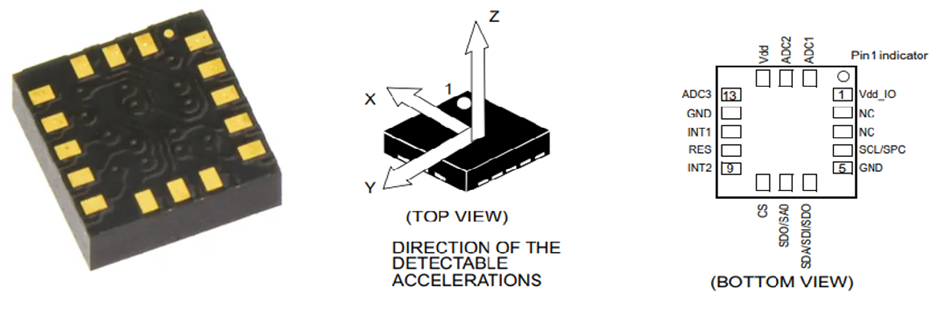
\includegraphics[width=0.8\textwidth]{images/lis.png}
		\caption{Cảm biến gia tốc LIS3DH và sơ đồ chân kết nối}
		\label{lis}
\end{figure}




\subsection{Vi xử lý}

Với sự phát triển vượt bậc và đa dạng của công nghệ chế tạo, 
có rất nhiều cấu hình phần cứng được nhiều nhóm tác giả lựa chọn phù 
hợp với các mục đích khác nhau. Trong đó, \cite{p_1} các tác giả đã 
sử dụng máy tính đơn Raspberry Pi kết hợp các điện trở cảm biến 
lực để phát hiện 4 tư thế ngủ với sự lấy nhãn từ video theo dõi người 
bệnh trong suốt quá trình lấy mẫu. Kwasnicki và cộng sự đã phát triển 
hệ thống ngủ có thể đeo (wearable sleep system) sử dụng bộ xử lý công 
suất thấp TI MSP430 và mô-đun RF Chipcon CC2420 cho truyền thông không 
dây kết hợp với cảm biến gia tốc 3 trục ADXL330, con quay hồi chuyển 
InvenSense ITG-3200, Honeywell HMC5843 để đo từ trường xác định 99.5\% 
chính xác 4 tư thế ngủ \cite{kwasnicki2018}. Tuy nhiên, các thiết bị vẫn 
yêu cầu một nguồn nặng lượng khiến cho tính liên tục bị hạn chế đáng kể. 
I.Yun và cộng sự đã phát triển thiết bị theo dõi tư thế ngủ của trẻ nhỏ 
sử dụng vi xử lý ATmega328P-PU cùng module Bluetooth kết hợp cảm biến gia 
tốc ADXL335 được đặt trên bụng đã nhưng lựa chọn về mặt cấu hình thiết bị 
và chế tạo ra mạch cung cấp năng lượng cho những thành phần cần thiết 
\cite{p_3}. Từ đó, giảm thiếu đáng kể mức tiêu thụ năng lượng và vẫn 
giữ nguyên độ chính xác nhưng khá bất tiện cho trẻ nhỏ. 
Trong nghiên cứu của Abdulsadig và cộng sự, 
hệ thống thu thập dữ liệu được xây dựng dựa trên một bo mạch tùy chỉnh tích 
hợp vi điều khiển nRF5232 (Nordic Semiconductor) – một SoC thuộc dòng 
ARM Cortex-M4F, hỗ trợ truyền thông không dây thông qua giao 
thức Bluetooth Low Energy (BLE). Vi điều khiển này đảm nhiệm đồng 
thời cả việc lấy mẫu dữ liệu từ cảm biến gia tốc ba trục LIS2DH12 
(STMicroelectronics) với tần số 100 Hz và truyền dữ liệu không dây 
theo thời gian thực \cite{Sleep_Posture_Detection, abdulsadig2023}. 
Trong nghiên cứu của Vũ Hoàng Diệu và cộng sự, 
mô-đun ESP32 được lựa chọn làm đơn vị xử lý trung tâm nhờ tích hợp bộ vi điều khiển hiệu năng cao, 
kết nối không dây Wi-Fi và khả năng mở rộng linh hoạt \cite{vu2023}. 
Với thiết kế nhỏ gọn, chi phí hợp lý và mức tiêu thụ điện năng thấp, 
ESP32 đáp ứng tốt yêu cầu của hệ thống thu thập dữ liệu tư thế ngủ theo 
thời gian thực. Thiết bị không chỉ cho phép truyền dữ liệu trực tiếp 
lên máy chủ hoặc nền tảng đám mây thông qua Wi-Fi, mà còn hỗ trợ 
lưu trữ cục bộ trên thẻ nhớ microSD, đảm bảo tính liên tục và 
an toàn dữ liệu trong điều kiện mất kết nối mạng.

Tuy nhiên, qua phân tích các nghiên cứu trên có thể thấy rằng phần 
lớn các cấu hình phần cứng hiện tại hoặc có chi phí triển khai cao, 
hoặc tiêu tốn năng lượng, hoặc gặp giới hạn trong khả năng tích hợp mô 
hình học máy tại thiết bị. Do đó, việc lựa chọn một kiến trúc vi xử lý 
vừa đảm bảo hiệu suất xử lý tín hiệu sinh lý thời gian thực, vừa tối 
ưu năng lượng và có khả năng triển khai mô hình TinyML là cần thiết. 
Trong số các kiến trúc hiện nay, dòng ARM Cortex-M4 nổi bật nhờ tính 
cân bằng giữa hiệu năng, mức tiêu thụ năng lượng thấp và khả năng hỗ 
trợ xử lý tín hiệu số, phù hợp với các hệ thống đeo được trong theo 
dõi tư thế ngủ.


Kiến trúc ARM có nhiều dòng vi xử lý khác nhau, được phát triển và nâng
cấp liên tục nhằm đáp ứng nhu cầu đa dạng trong lĩnh vực công nghệ nhúng. 
Trong đó, dòng Cortex-M thuộc kiến trúc ARMv7 đã trở thành nền tảng phổ 
biến cho các hệ thống nhúng sử dụng vi điều khiển nhờ vào hiệu suất cao, 
khả năng mở rộng và mức tiêu thụ năng lượng tối ưu. Dòng Cortex-M bao 
gồm nhiều phiên bản như Cortex-M0, Cortex-M0+, Cortex-M1, Cortex-M3, 
Cortex-M4 và Cortex-M7, mỗi phiên bản được thiết kế để phục vụ cho các mức 
độ yêu cầu hiệu năng khác nhau \cite{arm_cortex_m_comparison}. 
Các vi xử lý thuộc họ Cortex-M chủ yếu được ứng dụng trong các hệ thống 
nhúng thời gian thực, nơi yêu cầu sự cân bằng giữa hiệu suất xử lý, tiêu 
thụ năng lượng và chi phí. Một số vi xử lý ARM khác, không thuộc họ 
Cortex-M, được sử dụng trong các thiết bị hiệu suất cao như điện thoại 
thông minh và máy tính bảng, vốn yêu cầu cấu hình phần cứng mạnh hơn và 
khả năng xử lý đa tác vụ cao hơn.
Theo tài liệu \cite{cortexM4}, vi xử lý Cortex-M4 là một bộ xử lý 32-bit 
sử dụng kiến trúc tập lệnh rút gọn (RISC), được xây dựng theo kiến trúc 
Harvard, trong đó bus dữ liệu và bus lệnh được tách biệt nhằm tối ưu 
hiệu suất truy xuất bộ nhớ. Vi xử lý này hỗ trợ đầy đủ cả tập lệnh 
Thumb-1 (16-bit) và Thumb-2 (hỗn hợp 16/32-bit), mang lại sự linh hoạt 
trong mã hóa lệnh và tiết kiệm không gian bộ nhớ chương trình.

Về hiệu năng, Cortex-M4 đạt từ 1,25 đến 1,95 DMIPS/MHz (Dhrystone Million Instructions Per Second per MHz), cho thấy khả năng xử lý hiệu quả trong các ứng dụng nhúng yêu cầu độ chính xác và độ phản hồi thời gian thực cao. Bên cạnh đó, vi xử lý hỗ trợ tối đa 240 tín hiệu ngắt, bao gồm cả ngắt không thể bị chặn (Non-Maskable Interrupts – NMI), cùng khả năng cấu hình từ 8 đến 256 mức ưu tiên ngắt, giúp hệ thống hoạt động ổn định trong môi trường có nhiều sự kiện cạnh tranh đồng thời.
Ngoài ra, hiện nay ứng dụng trí tuệ nhân tạo (AI) tại thiết bị biên (Edge AI) đang ngày càng phổ biến, đặc biệt trong các lĩnh vực như nhà thông minh, thiết bị đeo, giám sát an ninh và công nghiệp 4.0. Với khả năng xử lý tín hiệu số (DSP) và hỗ trợ các mạng nơ-ron nhỏ gọn, các vi xử lý Cortex-M, đặc biệt là dòng Cortex-M4, đang được khai thác để triển khai các mô hình học sâu nhẹ (tinyML) ngay trên vi điều khiển \cite{electronics11162545}\cite{applicationCortexM4}.


\begin{figure}[!ht]
		\centering
 		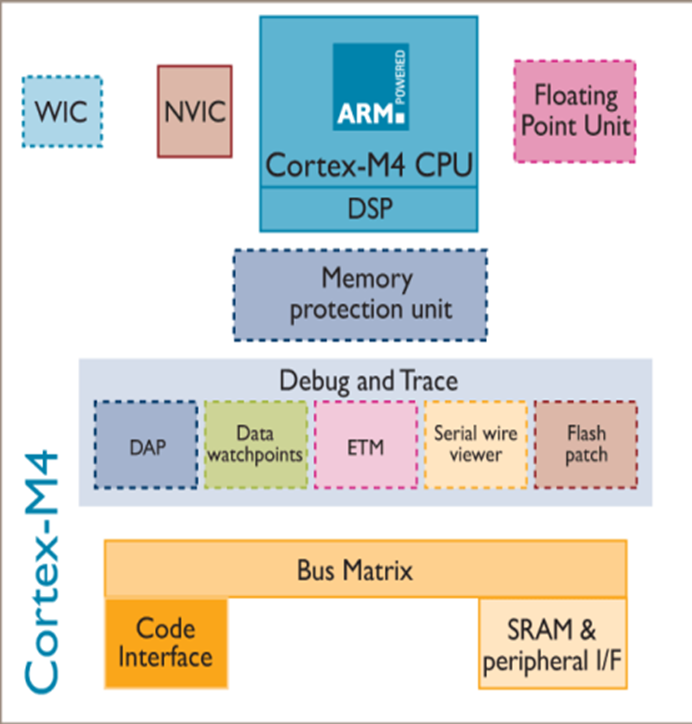
\includegraphics[width=0.8\textwidth]{images/cortexM4.png}
		\caption{Thành phần chính của vi điều khiển Cortex-M4}
		\label{cortexM4}
\end{figure}

Kết nối bus được mô tả trong Hình~\ref{cortexM4} cho phép truyền dữ liệu đồng thời trên nhiều bus khác nhau, đồng thời cung cấp khả năng quản lý truyền dữ liệu hiệu quả, chẳng hạn như sử dụng bộ đệm ghi và điều khiển hướng bit hoạt động (bit-banding). Hệ thống cũng có thể bao gồm các cầu bus (bus bridges) nhằm kết nối nhiều loại bus vào một mạng duy nhất sử dụng chung không gian bộ nhớ. Ngoài ra, bộ xử lý được trang bị hệ thống hỗ trợ gỡ lỗi tích hợp, bao gồm khả năng kiểm soát gỡ lỗi, thiết lập điểm ngắt (breakpoint) chương trình và điểm theo dõi dữ liệu (watchpoint). Khi xảy ra sự kiện gỡ lỗi, hệ thống có thể tạm dừng trạng thái hoạt động của lõi xử lý để phục vụ việc phân tích và xử lý lỗi.

Bên cạnh đó, kiến trúc Cortex-M4 tích hợp Bộ điều khiển ngắt vectored lồng nhau (Nested Vectored Interrupt Controller – NVIC) với khả năng hỗ trợ lên đến 240 tín hiệu yêu cầu ngắt, bao gồm cả ngắt không chắn được (NMI). NVIC hỗ trợ xử lý ngắt lồng nhau một cách tự động bằng cách so sánh mức ưu tiên giữa các yêu cầu ngắt với mức ưu tiên hiện tại đang được xử lý.

Đối với các ứng dụng yêu cầu tiết kiệm năng lượng, hệ thống còn được trang bị bộ đánh thức ngắt (Wake-up Interrupt Controller – WIC), cho phép đưa bộ vi điều khiển vào chế độ nghỉ bằng cách tắt hầu hết các thành phần không cần thiết, đồng thời duy trì khả năng đánh thức hệ thống khi phát hiện một yêu cầu ngắt. Ngoài ra, cơ chế bảo vệ bộ nhớ cũng được tích hợp nhằm đảm bảo an toàn cho hệ thống, ví dụ như chỉ cho phép truy cập đọc tại một số vùng bộ nhớ hoặc ngăn người dùng truy cập vào các vùng dữ liệu đặc quyền của hệ điều hành hoặc ứng dụng hệ thống.


\begin{figure}[!ht]
		\centering
 		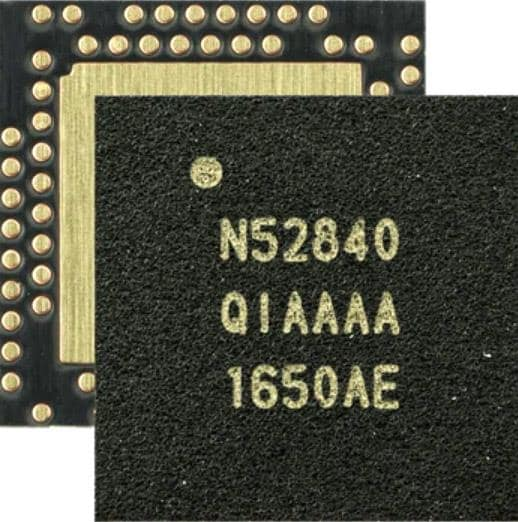
\includegraphics[width=0.8\textwidth]{images/NRF52840-QFA_SPL.jpg}
		\caption{Nordic Semiconductor NRF52840}
		\label{lis}
\end{figure}
Sau quá trình khảo sát và so sánh các dòng vi xử lý phổ biến, tác giả 
lựa chọn nRF52840 (Nordic Semiconductor) làm nền tảng phần cứng cho hệ 
thống đề xuất, nhờ vào các ưu điểm nổi bật như kích thước nhỏ, 
tiêu thụ năng lượng thấp và tích hợp sẵn giao tiếp Bluetooth Low Energy 
(BLE). Đây là vi xử lý cao cấp nhất trong dòng nRF52, thuộc loại hệ thống 
trên một vi mạch (System-on-Chip – SoC), được thiết kế chuyên biệt cho 
các ứng dụng không dây tầm ngắn và tiết kiệm năng lượng \cite{nrf52840}.

\textbf{nRF52840} tích hợp bộ thu phát đa giao thức hoạt động ở băng tần 2.4 GHz 
và bộ xử lý trung tâm Arm Cortex-M4F chạy ở xung nhịp 64 MHz, 
kèm bộ xử lý dấu phẩy động (FPU). Vi xử lý này được trang bị bộ nhớ 
1 MB Flash và 256 KB RAM, hỗ trợ chuẩn Bluetooth 5.3 cùng khả năng giao 
tiếp đa giao thức (multiprotocol), cho phép cải thiện tốc độ, phạm vi 
truyền và độ tin cậy của kết nối không dây. Hệ thống bảo mật tích hợp 
đầy đủ, bao gồm các tính năng mã hóa phần cứng, đáp ứng yêu cầu khắt khe 
về bảo vệ dữ liệu. Ngoài khả năng hoạt động trong dải điện áp rộng 
từ +1.7 V đến +5.5 V (tương thích với nguồn pin và USB), nRF52840 còn 
cung cấp các giao tiếp ngoại vi phong phú: tối đa hai giao diện I2C, 
bốn SPI master, ba SPI slave, bốn kênh PWM hỗ trợ EasyDMA, cùng với 
năm bộ định thời 32-bit, phù hợp cho các ứng dụng đòi hỏi xử lý thời 
gian thực chính xác. Tất cả các đặc điểm trên khiến nRF52840 trở thành 
lựa chọn lý tưởng cho các hệ thống nhúng đeo được tích hợp AI nhẹ và 
kết nối không dây thông minh.

Ngoài ra, nRF52840 hỗ trợ một hệ sinh thái phần mềm mạnh mẽ, bao gồm SDK 
của Nordic và nền tảng TensorFlow Lite for Microcontrollers, giúp rút 
ngắn thời gian phát triển và triển khai hệ thống TinyML. Thiết bị còn 
sở hữu khả năng quản lý năng lượng linh hoạt, tương thích tốt với nguồn pin hoặc USB. 





\subsection{Bluetooth năng lượng thấp}

Với mục tiêu tối ưu hóa năng lượng và đảm bảo khả năng hoạt động lâu dài 
cho thiết bị đeo sử dụng pin, Bluetooth Low Energy (BLE) được lựa chọn 
làm chuẩn kết nối không dây chính trong hệ thống phần cứng.

\begin{figure}[!ht]
		\centering
 		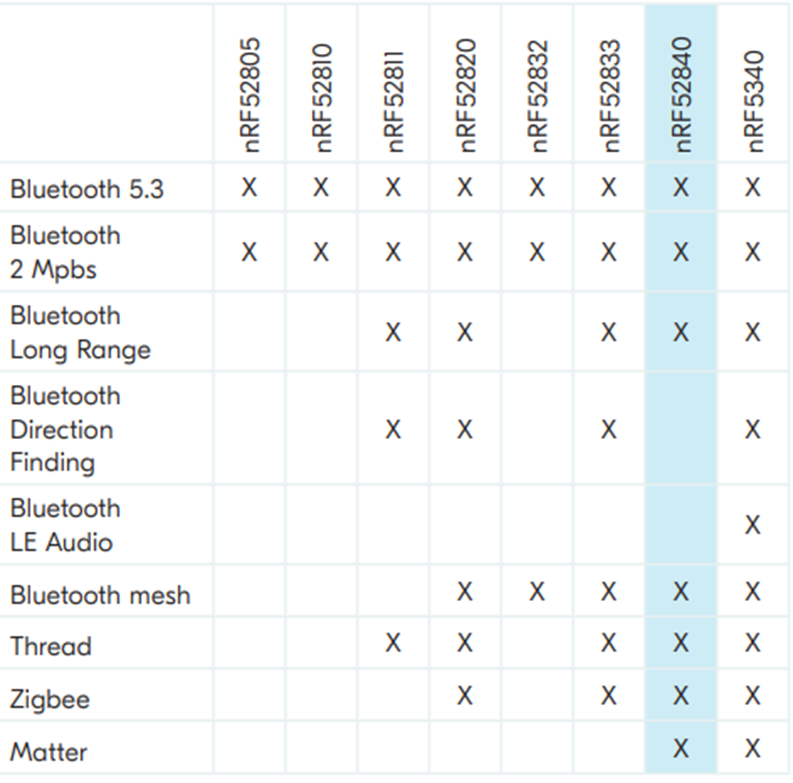
\includegraphics[width=0.8\textwidth]{images/ble.png}
		\caption{Các kiểu kết nối không dây trong họ chip nRF52}
		\label{ble}
\end{figure}

BLE là giao thức kết nối không dây được thiết kế chuyên biệt cho 
các ứng dụng năng lượng thấp, hoạt động ở băng tần ISM 2.4 GHz, 
hỗ trợ thông lượng ứng dụng lên đến 1.4 Mbps. Với ưu thế tiêu thụ năng 
lượng tối thiểu nhưng vẫn đảm bảo tốc độ truyền phù hợp, BLE đặc biệt 
thích hợp cho các thiết bị y sinh hoạt động liên tục bằng pin có dung 
lượng hạn chế. BLE hiện được hỗ trợ phổ biến trên hầu hết các hệ điều 
hành như iOS, Android, macOS, Windows 10 và Linux, cũng như trong các 
thiết bị di động hiện đại.

Về mặt bảo mật, BLE tích hợp các cơ chế mã hóa và xác thực nhằm đảm bảo 
tính bí mật, toàn vẹn và riêng tư của dữ liệu truyền qua mạng. 
Công nghệ này đã trở thành một phần tiêu chuẩn trong hầu hết các 
thiết bị di động hiện đại như smartphone, máy tính bảng, và laptop, 
đồng thời được hỗ trợ đầy đủ trên các hệ điều hành phổ biến bao gồm iOS, 
Android, macOS, Windows 10 và Linux. Bluetooth 5 là bước phát triển 
đột phá tiếp theo kể từ khi BLE được giới thiệu trong chuẩn Bluetooth 
4.0, mang đến hàng loạt cải tiến đáng kể giúp mở rộng phạm vi ứng dụng 
và nâng cao hiệu suất hệ thống. Một trong những cải tiến nổi bật là 
chế độ 2 Mbps, cho phép tăng gấp đôi tốc độ truyền lý thuyết, tương 
ứng với thông lượng thực tế lên đến 1.4 Mbps. Quan trọng hơn, chế độ 
này còn giúp giảm đáng kể mức tiêu thụ năng lượng – cụ thể là giảm một 
nửa năng lượng tiêu thụ trên mỗi bit dữ liệu – từ đó kéo dài thời gian 
hoạt động của thiết bị hoặc cho phép sử dụng các nguồn năng lượng nhỏ 
và chi phí thấp hơn \cite{BLE}. 

Bên cạnh đó, tính năng Advertising Extensions (mở rộng quảng cáo) đã 
cách mạng hóa cơ chế phát sóng của BLE. Các gói quảng cáo giờ đây có 
thể chứa lượng dữ liệu gấp 8 lần so với phiên bản trước, cho phép 
truyền tải các khối dữ liệu lớn hơn mà không cần thiết lập kết nối 
ngay lập tức. Đồng thời, các gói quảng cáo có thể được xâu chuỗi 
để tạo thành các tập tin quảng cáo phức hợp. Tính năng lựa chọn kênh 
được tối ưu hóa giúp tăng cường độ ổn định và khả năng chống nhiễu 
trong các môi trường có mật độ thiết bị cao. Đặc biệt, chế độ Long 
Range mở rộng đáng kể phạm vi truyền thông của BLE, cho phép các thiết 
bị duy trì kết nối trong toàn bộ không gian của một ngôi nhà thông minh 
hoặc trong các ứng dụng IoT công nghiệp quy mô vừa và nhỏ.




\begin{figure}[!ht]
	\centering
 	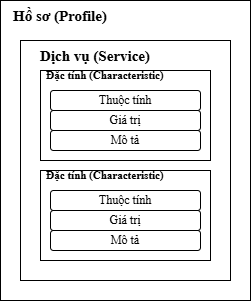
\includegraphics[width=0.5\textwidth]{images/gatt.drawio.png}
	\caption{Cấu trúc của GATT}
	\label{gatt}
\end{figure}

BLE tổ chức logic giao tiếp dựa trên mô hình GATT 
(Generic Attribute Profile). GATT quy định cách hai thiết bị BLE 
trao đổi dữ liệu thông qua các đơn vị logic: dịch vụ (services) 
và đặc tính (characteristics). Giao thức nền tảng là Attribute Protocol 
(ATT) – nơi mỗi đặc tính được định danh bằng UUID 16-bit hoặc 128-bit, 
với quyền truy cập như chỉ đọc, chỉ ghi, hoặc hỗ trợ thông báo (notify).

Một điểm quan trọng trong mô hình GATT là tính kết nối độc quyền: 
tại một thời điểm, thiết bị ngoại vi chỉ có thể duy trì một kết nối 
duy nhất với thiết bị trung tâm. Khi kết nối được thiết lập, thiết bị 
ngừng quảng cáo, điều này hạn chế khả năng kết nối đồng thời từ 
nhiều thiết bị.

Ngoài ra, vi xử lý nRF52840 còn hỗ trợ Bluetooth Mesh, cho phép thiết 
lập mạng lưới nhiều-nút (many-to-many), sử dụng BLE làm lớp truyền tải 
vật lý. Mỗi nút trong mạng có thể đóng vai trò chuyển tiếp (relay), 
cho phép dữ liệu lan truyền đến các vùng rộng hơn theo mô hình phân 
tán – phù hợp với các ứng dụng IoT quy mô lớn như nhà thông minh, 
chiếu sáng công nghiệp hoặc giám sát phân tán. Trong mạng Mesh, 
các gói dữ liệu có thể được đóng gói qua advertising packet hoặc 
qua các giao tiếp GATT tùy tình huống sử dụng.

Các profile BLE là tập hợp các dịch vụ được chuẩn hóa bởi Bluetooth 
SIG hoặc định nghĩa tùy chỉnh, ví dụ như dịch vụ UART tùy chỉnh gồm 
hai đặc tính RX và TX, tương ứng với kênh nhận và truyền.

\subsection{Thiết bị thực nghiệm}
Trong khuôn khổ của khóa luận, nhằm đảm bảo tiến độ triển khai và tính an 
toàn trong giai đoạn thử nghiệm, tác giả lựa chọn sử dụng bộ kit thương 
mại Adafruit Playground để tiến hành thực nghiệm sơ bộ. Bộ kit này tích 
hợp sẵn cảm biến gia tốc MEMS LIS3DH được gắn tại vị trí trung tâm, 
cho phép đo gia tốc theo ba trục không gian X, Y và Z với độ chính xác cao. 
Theo tài liệu từ nhà sản xuất, chi phí cho mỗi bộ kit Adafruit vào khoảng 
25 USD \cite{ada_overview}. Trong bộ kit, cảm biến LIS3DH được kết nối với 
vi điều khiển thông qua giao thức SPI, với chân chọn thiết bị (CS) được 
gán tại chân số 8 và đầu ra ngắt tùy chọn (IRQ) tại chân số 7 (IRQ \#4). 
Theo sơ đồ bố trí tiêu chuẩn của kit, trục X định hướng theo chiều giắc 
USB, trục Y hướng sang bên trái, và trục Z vuông góc theo hướng mặt trên 
của thiết bị.

Bên cạnh đó, để mở rộng khả năng nghiên cứu và đánh giá tính khả thi khi 
tích hợp học máy nhẹ (TinyML) cũng như kết nối không dây, nhóm nghiên 
cứu sử dụng thêm nền tảng Arduino Nano 33 BLE Sense. Đây là vi điều khiển 
hiện đại tích hợp vi xử lý nRF52840 (ARM Cortex-M4F), hỗ trợ Bluetooth 
Low Energy (BLE) và nhiều cảm biến tích hợp (IMU, microphone, nhiệt độ, 
độ ẩm, v.v.), đồng thời tương thích với nền tảng TensorFlow Lite for 
Microcontrollers \cite{nano33ble}.

Đáng chú ý, bên cạnh việc sử dụng các bộ kit sẵn có, một thành viên khác 
trong nhóm đang tiến hành phát triển và xây dựng bản mạch phần cứng 
tùy chỉnh dựa trên các thông số kỹ thuật đã được phân tích ở các phần 
trước. Hướng tiếp cận này không chỉ giúp nhóm triển khai nhanh chóng hệ 
thống thử nghiệm trong giai đoạn đầu, mà còn mở ra khả năng thiết kế một 
thiết bị nhúng chuyên dụng, tối ưu hơn về chi phí, hiệu năng và khả năng 
tích hợp trong các ứng dụng thực tiễn.


\begin{figure}[!ht]
		\centering
 		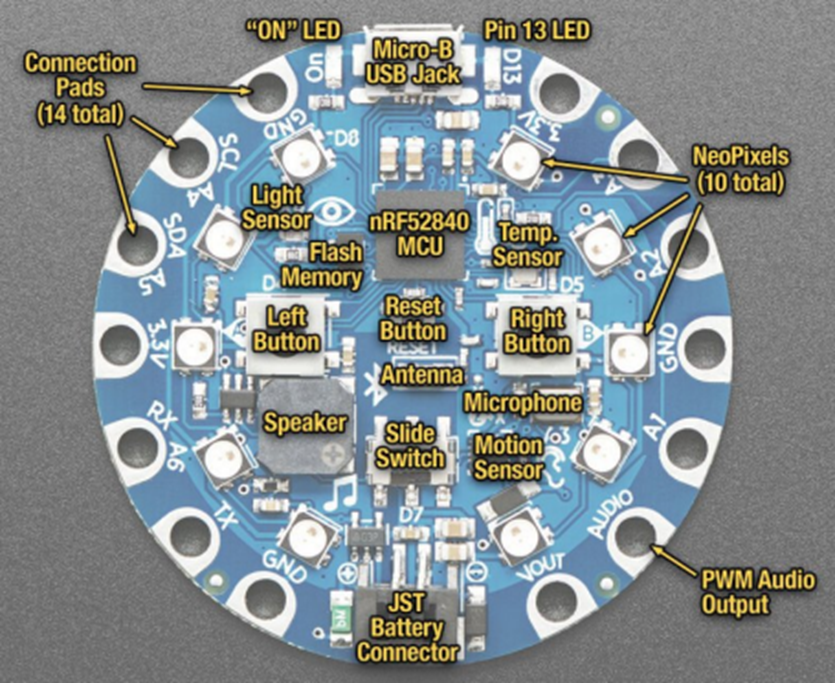
\includegraphics[width=0.8\textwidth]{images/detail_ada.png}
		\caption{Cấu trúc các thành phần trên Circuit PlayGround}
		\label{detail_ada}
\end{figure}





\section{Hệ thống thu thập, xử lý, lưu trữ dữ liệu}
Phần này trình bày tổng quan kiến trúc hệ thống bao gồm: 
lập trình firmware trên vi điều khiển để thu thập dữ liệu cảm biến, 
thiết kế ứng dụng di động làm cầu nối giữa phần cứng và hệ thống đám mây, 
cùng với backend và cơ sở dữ liệu lưu trữ phục vụ huấn luyện mô hình. 
Nội dung cũng đề cập đến các yêu cầu chức năng, phi chức năng và 
thiết kế hệ thống ở mức cao nhằm đảm bảo khả năng triển khai thực 
tế và mở rộng trong tương lai.


\subsection{Lập trình vi xử lý}

Thiết bị được lập trình trên nền tảng Arduino IDE, sử dụng thư viện 
\texttt{Adafruit Circuit Playground}. Trong hàm \texttt{setup()}, 
thiết bị khởi tạo các bản tin quảng cáo (advertising), 
cấu hình kết nối/ngắt kết nối, và thiết lập cấu trúc dịch vụ theo 
giao thức \gls{GATT} của BLE, như được minh họa trong Hình~\ref{flowBLE}.

\begin{figure}[htbp]
    \centering
    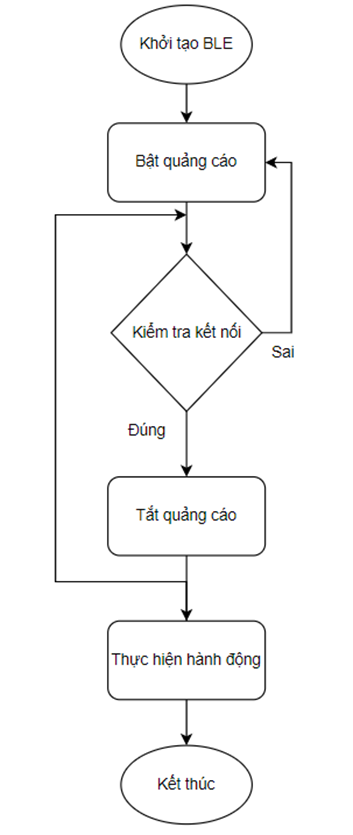
\includegraphics[width=0.5\textwidth]{images/flowBLE.png}
    \caption{Lưu đồ hoạt động của thiết bị BLE}
    \label{flowBLE}
\end{figure}

Trong đoạn mã~\ref{arduinoBLE}, hàm \texttt{startAdv()} đảm nhiệm cấu 
hình quảng bá BLE cho thiết bị. Quá trình này bao gồm: thiết lập cờ 
kết nối tổng quát, chèn thông tin công suất truyền (Tx Power), 
thêm UUID của dịch vụ tư thế (\texttt{positionService}) và tên thiết 
bị vào gói quảng bá. Các thông số quảng bá được cấu hình theo khuyến 
nghị của Apple nhằm đảm bảo khả năng tương thích với thiết bị iOS: 
chế độ nhanh với chu kỳ 20ms, chế độ chậm 152.5ms, và thời gian chuyển 
chế độ sau 30 giây. Thiết bị sẽ tiếp tục phát tín hiệu quảng bá cho 
đến khi có kết nối được thiết lập.

Trong cấu trúc dịch vụ, tác giả định nghĩa một dịch vụ chính với UUID 
là \texttt{0x1821}, kèm theo hai đặc tính cảm biến: gia tốc 
(\texttt{UUID 0x2713}, đơn vị \texttt{m/s\textsuperscript{2}}) và 
gia tốc góc (\texttt{UUID 0x2744}, 
đơn vị \texttt{rad/s\textsuperscript{2}}). 
Tuy hệ thống hỗ trợ cả hai loại dữ liệu, trong khuôn khổ khoá luận này, 
tác giả chỉ tập trung vào giá trị gia tốc thu được từ cảm biến để phục 
vụ bài toán phân loại tư thế ngủ.

\begin{lstlisting}[float,language=C,caption=Tập lệnh khởi tạo và kết nối Bluetooth từ thư viện của AdaFruit, label=arduinoBLE,captionpos=b]
void startAdv(void)
{
  // Advertising packet
  Bluefruit.Advertising.addFlags(BLE_GAP_ADV_FLAGS_LE_ONLY_GENERAL_DISC_MODE);
  Bluefruit.Advertising.addTxPower();

  // Include HRM Service UUID
  Bluefruit.Advertising.addService(positionService);

  // Include Name
  Bluefruit.Advertising.addName();
  
  /* Start Advertising
   * - Enable auto advertising if disconnected
   * - Interval:  fast mode = 20 ms, slow mode = 152.5 ms
   * - Timeout for fast mode is 30 seconds
   * - Start(timeout) with timeout = 0 will advertise forever (until connected)
   * 
   * For recommended advertising interval
   * https://developer.apple.com/library/content/qa/qa1931/_index.html   
   */
  Bluefruit.Advertising.restartOnDisconnect(true);
  Bluefruit.Advertising.setInterval(32, 244);    // in unit of 0.625 ms
  Bluefruit.Advertising.setFastTimeout(30);      // number of seconds in fast mode
  Bluefruit.Advertising.start(0);                // 0 = Don't stop advertising after n seconds  
}
\end{lstlisting}


\begin{lstlisting}[float,language=C,caption=Gửi dữ liệu từ BLE, label=sendBle,captionpos=b]
void setupPosition(void)
{
 
  positionService.begin();

  accelerometerCharacter.setProperties(CHR_PROPS_NOTIFY+CHR_PROPS_READ+CHR_PROPS_WRITE );
  accelerometerCharacter.setPermission(SECMODE_OPEN, SECMODE_NO_ACCESS);
  accelerometerCharacter.setFixedLen(9);
  accelerometerCharacter.setCccdWriteCallback(cccd_callback);  // Optionally capture CCCD updates
  accelerometerCharacter.begin();
  uint8_t accelerometerData[9] = { 0b00000000, 0b00000000, 0b00000000,0b00000000,0b00000000,0b00000000,0b00000000,0b00000000,0b00000000}; // Set the characteristic to use 8-bit values, with the sensor connected and detected
  accelerometerCharacter.write(accelerometerData, 9);

  gyroscopeCharacter.setProperties(CHR_PROPS_READ);
  gyroscopeCharacter.setPermission(SECMODE_OPEN, SECMODE_NO_ACCESS);
  gyroscopeCharacter.setFixedLen(1);
  gyroscopeCharacter.begin();
  gyroscopeCharacter.write8(2);    // Set the characteristic to 'Wrist' (2)
}

\end{lstlisting}

Ngoài các thao tác khởi tạo dịch vụ, thư viện BLE của Adafruit còn cung cấp các phương thức cấu hình đặc tính (\textit{characteristics}) nhằm kiểm soát hành vi và bảo mật của kết nối BLE.

Cụ thể, phương thức \texttt{setProperties} cho phép cấu hình quyền truy cập của đặc tính, với các lựa chọn phổ biến như:

\begin{description}
    \item[\texttt{CHR\_PROPS\_BROADCAST}] phát sóng đặc tính (bit 0)
    \item[\texttt{CHR\_PROPS\_READ}] cho phép thiết bị đọc (bit 1)
    \item[\texttt{CHR\_PROPS\_WRITE\_WO\_RESP}] ghi không cần phản hồi (bit 2)
    \item[\texttt{CHR\_PROPS\_WRITE}] ghi với phản hồi (bit 3)
    \item[\texttt{CHR\_PROPS\_NOTIFY}] gửi thông báo không xác nhận (bit 4)
    \item[\texttt{CHR\_PROPS\_INDICATE}] gửi thông báo có xác nhận (bit 5)
\end{description}

Ngoài ra, một số phương thức bổ trợ khác bao gồm:

\begin{description}
    \item[\texttt{setPermission}] thiết lập quyền truy cập và mức độ bảo mật (ví dụ: không cần xác thực, cần mã hoá, v.v.)
    \item[\texttt{setFixedLen}] xác định độ dài cố định của dữ liệu truyền
\end{description}

\begin{figure}[htbp]
    \centering
    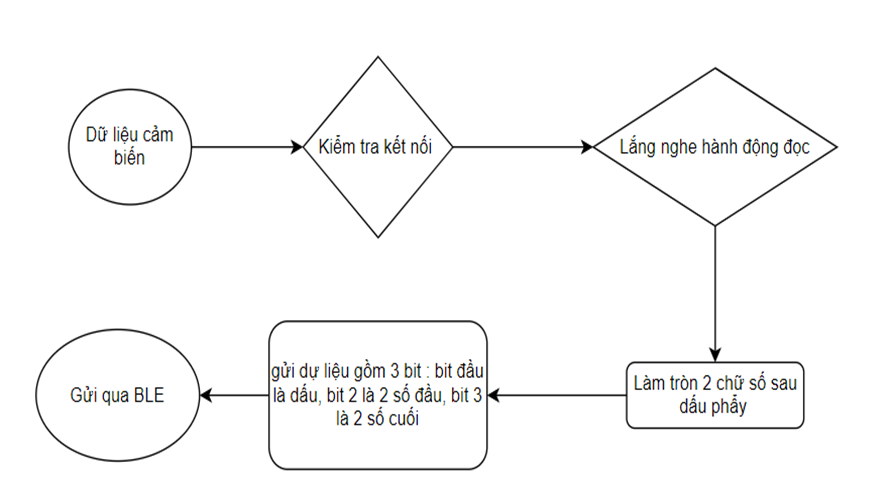
\includegraphics[width=\textwidth]{images/sendBleFlow.png}
    \caption{Lưu đồ luồng gửi thông tin BLE}
    \label{sendBleFlow}
\end{figure}


Luồng xử lý dữ liệu BLE được minh hoạ tại Hình~\ref{sendBleFlow}. 
Sau khi thu nhận dữ liệu cảm biến, thiết bị kiểm tra trạng thái 
kết nối BLE. Nếu kết nối hợp lệ, nó sẽ tiếp tục lắng nghe hành động đọc 
từ phía thiết bị trung tâm. Dữ liệu sau đó được làm tròn đến hai chữ số 
thập phân và mã hoá thành ba byte: byte đầu tiên lưu dấu, byte thứ hai 
chứa hai chữ số đầu, và byte cuối là hai chữ số cuối của giá trị gia tốc. 
Chuỗi dữ liệu này được gửi qua BLE theo đặc tính đã định nghĩa trước đó.














\subsection{Hiệu chuẩn cảm biến}
Việc thu nhận và tiền xử lý dữ liệu là bước quan trọng trong các hệ đo 
lường. Mặc dù cảm biến thường được hiệu chuẩn từ nhà sản xuất, nhưng 
vẫn cần được hiệu chuẩn lại trong môi trường đo thực tế để cải thiện 
hiệu năng và giảm thiểu sai số. Các sai số này được chia thành hai 
loại chính: (i) sai số hệ thống (mặc định) và (ii) sai số ngẫu nhiên.

\textbf{Hiệu chuẩn sai số hệ thống.} Tác giả sử dụng gia tốc trọng trường 
để hiệu chuẩn cảm biến theo hướng tĩnh. Khi xoay cảm biến sao cho một 
trục hướng lên vuông góc với mặt phẳng nằm ngang, giá trị đo được 
là $-1g$; khi hướng xuống dưới, giá trị là $+1g$. Bằng cách xoay cảm 
biến lần lượt qua sáu vị trí tĩnh tương ứng với các hướng trục chính, 
có thể xác định được các điểm chuẩn, từ đó nội suy để xác định giá 
trị $0g$ một cách chính xác và đáng tin cậy.

\begin{figure}[htbp]
    \centering
    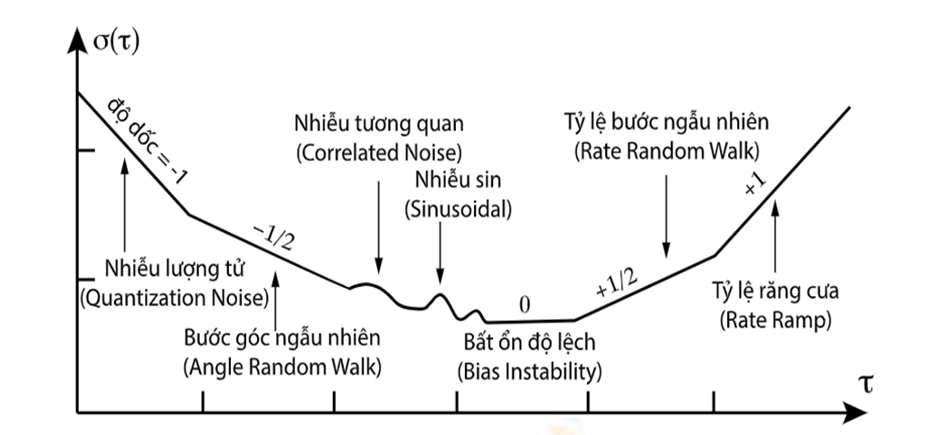
\includegraphics[width=\textwidth]{images/allan.png}
    \caption{Minh hoạ kết quả phân tích đường cong Allan}
    \label{allan}
\end{figure}

\textbf{Phân tích sai số ngẫu nhiên.} Tác giả sử dụng phương sai Allan 
để phân tích các thành phần nhiễu trong dữ liệu cảm biến \cite{allan}. 
Đây là phương pháp phân tích miền thời gian phổ biến nhằm đánh giá độ 
ổn định tần số và định lượng các loại nhiễu khác nhau như nhiễu trắng, 
trôi ngẫu nhiên, và nhiễu lượng tử. Biểu đồ Allan log-log cho phép nhận 
diện các thành phần nhiễu thông qua độ dốc của từng đoạn đường cong.

Trong thử nghiệm, cảm biến được đặt cố định trong phòng ở điều kiện 
nhiệt độ ổn định, với tần số lấy mẫu 10 Hz, thu được tổng cộng 1.211.210 
mẫu. Kết quả biểu diễn trong Hình~\ref{allan_real} cho thấy nhiễu chiếm 
ưu thế là nhiễu lượng tử (quantization noise), đặc trưng bởi hệ số góc 
tương ứng trong đồ thị.



\begin{figure}[htbp]
    \centering
    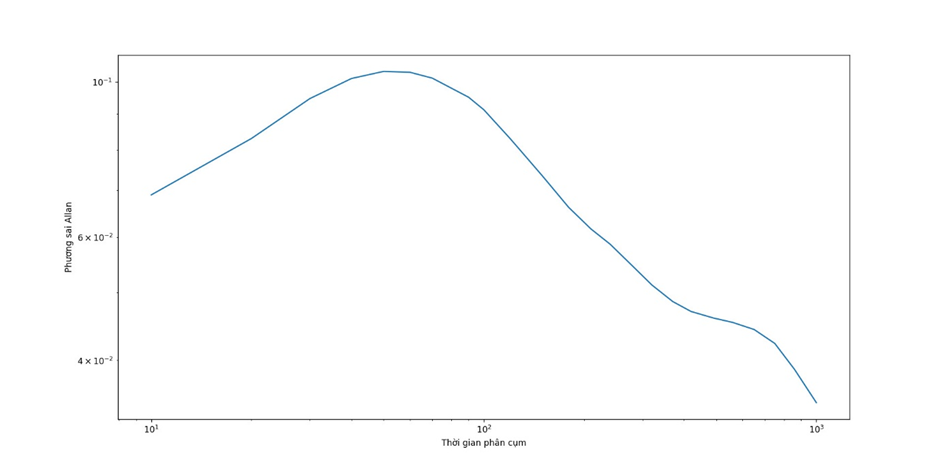
\includegraphics[width=\textwidth]{images/allan_real.png}
    \caption{Biểu đồ phương sai Allan của trục X}
    \label{allan_real}
\end{figure}

\textbf{Lọc nhiễu bằng bộ lọc Kalman.} Để xử lý nhiễu, đặc biệt là nhiễu 
lượng tử, tác giả sử dụng bộ lọc Kalman \cite{kalman}. Đây là một bộ lọc 
đệ quy có khả năng ước lượng trạng thái tối ưu của hệ thống từ các chuỗi 
đo lường bị nhiễu. Bộ lọc Kalman không chỉ phù hợp cho hệ thống tuyến 
tính mà còn có thể áp dụng cho hệ thống phi tuyến thông qua tuyến tính 
hoá cục bộ.

Trong hệ thống đề xuất, tín hiệu sau khi được cảm biến thu nhận sẽ 
được lọc trực tiếp tại vi điều khiển trước khi truyền đến ứng dụng 
để hiển thị và lưu trữ. Kết quả sau lọc được minh hoạ trong 
Hình~\ref{kalman}, cho thấy sự cải thiện đáng kể về độ mượt và ổn 
định của tín hiệu.


\begin{figure}[htbp]
    \centering
    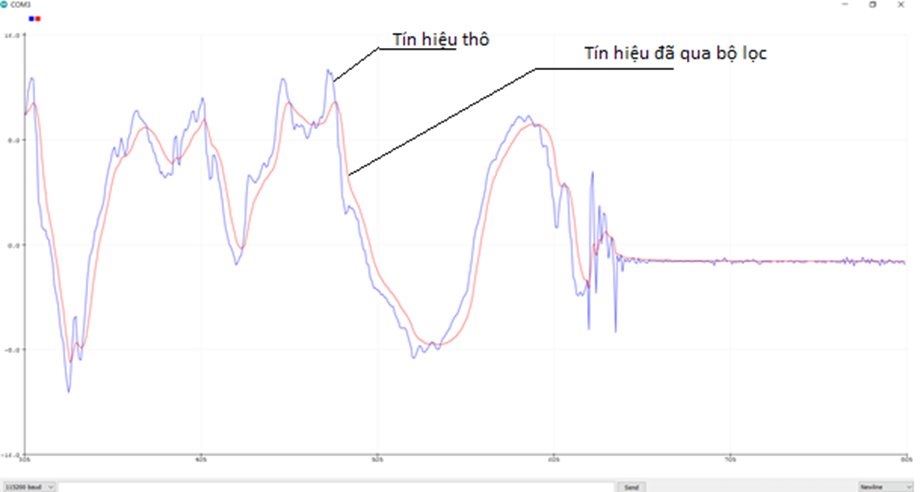
\includegraphics[width=\textwidth]{images/kalman.png}
    \caption{Kết quả bộ lọc Kalman cho dữ liệu trục X của cảm biến gia tốc}
    \label{kalman}
\end{figure}





\subsection{Xây dựng phần mềm ứng dụng}

Phần mềm ứng dụng được xây dựng với mục tiêu hỗ trợ người dùng trong việc 
kết nối với thiết bị phần cứng và trực quan hoá dữ liệu cảm biến. 
Ứng dụng đảm nhiệm vai trò là cầu nối giữa người dùng và hệ thống nhúng, 
đồng thời cung cấp các chức năng tương tác, cấu hình và theo dõi dữ liệu 
theo thời gian thực.

Các công nghệ và thành phần sử dụng được tóm tắt như sau:

\begin{flushleft}
\textbf{01)} Ngôn ngữ lập trình: \texttt{Dart} \\
\textbf{02)} Framework: \texttt{Flutter} \\
\textbf{03)} Nền tảng triển khai: \texttt{Android} \\
\textbf{04)} Giao tiếp phần cứng: Bluetooth Low Energy (BLE) \\
\textbf{05)} Chức năng chính: kết nối thiết bị, nhận dữ liệu, hiển thị, lưu trữ và cá nhân hóa trải nghiệm người dùng
\end{flushleft}

\begin{figure}[htbp]
    \centering
    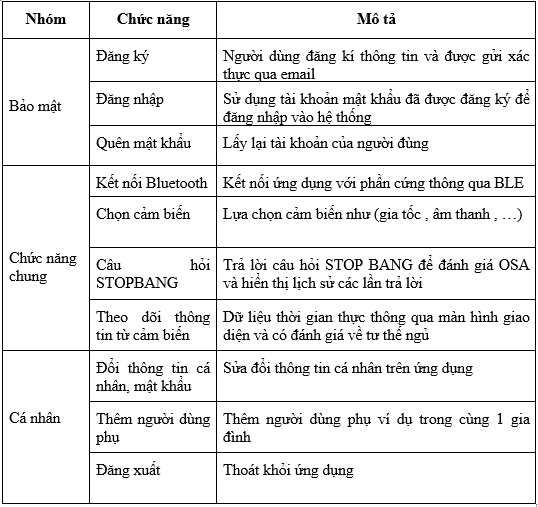
\includegraphics[width=\textwidth]{images/app_flow.png}
    \caption{Các nhóm chức năng chính của ứng dụng}
    \label{app_flow}
\end{figure}

Ứng dụng được thiết kế xoay quanh ba nhóm chức năng chính như minh họa 
trong Hình~\ref{app_flow}:

\begin{flushleft}
\textbf{01)} Nhóm bảo mật: đăng nhập, xác thực và khôi phục tài khoản. \\
\textbf{02)} Nhóm chức năng chung: kết nối với thiết bị phần cứng, thu thập và hiển thị dữ liệu cảm biến. \\
\textbf{03)} Nhóm cá nhân hoá: theo dõi chỉ số sức khỏe, khai báo STOP-BANG, lưu hồ sơ người dùng.
\end{flushleft}

\subsubsection*{Kiến trúc phần mềm}
Ứng dụng sử dụng mô hình \textbf{BLoC (Business Logic Component)} để tách biệt giao diện 
người dùng và logic xử lý. BLoC hoạt động dựa trên nguyên tắc nhận sự 
kiện đầu vào và trả về trạng thái phù hợp, giúp quản lý luồng dữ liệu 
hiệu quả. Cấu trúc tổng thể của kiến trúc BLoC gồm ba lớp chính được mô 
tả trong Hình~\ref{flutter}.

\begin{figure}[htbp]
    \centering
    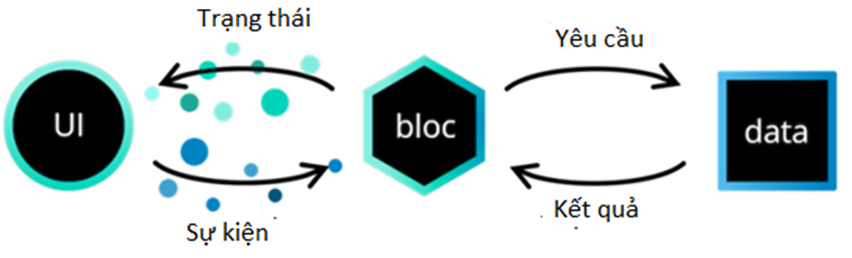
\includegraphics[width=0.8\textwidth]{images/flutter.png}
    \caption{Cấu trúc kiến trúc BLoC trong ứng dụng Flutter}
    \label{flutter}
\end{figure}


\begin{lstlisting}[float,language=dart,caption=Tập lệnh để tìm kiểm dịch vụ cảm biến ,label=flutterBle,captionpos=b]
StreamBuilder<List<BluetoothService>>(
      stream: device.services,
      initialData: [],
      builder: (c, snapshot) {
        if (snapshot.data!.length > 0) {
          isService = true;
        }
        BluetoothService serviceAcclerometer;
        if (snapshot.data == null || snapshot.data!.length == 0) {
          return Text("Please contact customer Service");
        }
        for (int i = 0; i < snapshot.data!.length; i++) {
          if (snapshot.data![i].uuid.toString() ==
              Constants.ACCLEROMETER_SERVICE) {
            accelerometerService = snapshot.data![i];
           }
        }
        if (accelerometerService == null) {
          return Text("Please contact customer Service");
        }
        for (int i = 0;
            i < accelerometerService!.characteristics.length;
            i++) {
          print(accelerometerService!.characteristics[i].uuid);
          if (accelerometerService!.characteristics[i].uuid
                  .toString() ==
              Constants.ACCLEROMETER_CHARACTION) {
            accelerometerCharactis =
                accelerometerService!.characteristics[i];
          }
        }
}));

\end{lstlisting}

\begin{lstlisting}[float,language=C,caption="Cấu trúc dữ liệu của phần nội dung đẩy lên máy chủ",label=format_ble,captionpos=b]
{
    "value": "0.88%0.66%0.99@2022-01-01/0.88%0.66%0.99@2022-01-01/0.88%0.66%0.99@2022-01-01",
    "customer": "62a5f5672ad9c724ef117d76"
}

\end{lstlisting}


Sau khi kết nối BLE được thiết lập thành công, ứng dụng truy xuất đối tượng đặc 
tính cảm biến (characteristic instance) và liên tục gửi yêu cầu đọc (\texttt{read}) 
đến vi điều khiển. Thiết bị phản hồi bằng cách trả về dữ liệu cảm biến 
dưới dạng mảng \texttt{UInt8}. Các giá trị này được ứng dụng giải mã, 
chuyển đổi sang dạng số thực tương ứng với gia tốc trên ba trục (X, Y, Z), 
và gắn nhãn thời gian thực.

Quá trình xử lý này được thực hiện trong một vòng 
lặp có kiểm soát độ trễ ngắn nhằm đảm bảo khả năng cập nhật liên tục 
nhưng vẫn tối ưu hiệu suất hệ thống.

Mã~\ref{flutterBle} minh hoạ toàn bộ quy trình xử lý: 
từ kết nối BLE, truy xuất đặc tính gia tốc, đọc giá trị nhị phân 
thô từ thiết bị, đến việc chuẩn hoá và gửi dữ liệu lên backend. 
Trong đoạn mã này, dữ liệu dạng \texttt{Uint8List} nhận từ cảm biến được tách và chuyển đổi 
thành ba thành phần tương ứng với ba trục gia tốc. Dữ liệu sau khi được xử lý sẽ được 
đóng gói theo định dạng \texttt{JSON} và gửi đến máy chủ thông qua phương thức 
POST, sử dụng thư viện \texttt{http} trong Flutter.

Định dạng dữ liệu BLE được chuẩn hoá như trong Mã~\ref{format_ble}, 
với trường \texttt{"value"} là chuỗi liên tục các 
giá trị cảm biến (phân tách bằng ký tự đặc biệt) và trường 
\texttt{"customer"} để định danh người dùng.

Việc tối ưu hóa cả quá trình đọc BLE và đẩy dữ liệu HTTP theo lô 
như vậy giúp giảm độ trễ, tránh tình trạng nghẽn băng thông, đồng thời 
vẫn đảm bảo độ chính xác và toàn vẹn của dữ liệu cảm biến.


Ngoài các chức năng thu thập và truyền dữ liệu cảm biến, ứng dụng còn tích hợp 
các công cụ hỗ trợ đánh giá y học lâm sàng ban đầu nhằm phục vụ cho việc sàng 
lọc và phân loại nguy cơ mắc hội chứng ngưng thở khi ngủ (OSA). Trong đó, 
ba thành phần quan trọng được triển khai bao gồm:

\noindent\textbf{01)} Bộ câu hỏi \textbf{STOP-BANG}: Đây là một bảng sàng lọc lâm sàng được sử dụng phổ biến trong y học giấc ngủ để đánh giá nguy cơ mắc OSA. Dữ liệu từ bảng này được lưu trữ cùng với dữ liệu cảm biến và đóng vai trò như đầu vào bổ sung cho các mô hình học máy dự đoán chỉ số AHI (Apnea–Hypopnea Index).

\vspace{0.5em}
\noindent\textbf{02)} Thang điểm \textbf{Epworth Sleepiness Scale (ESS)}: Tác giả triển khai thêm bảng câu hỏi ESS nhằm đánh giá mức độ buồn ngủ ban ngày của người dùng. Thang điểm này giúp phát hiện tình trạng buồn ngủ quá mức và có thể hỗ trợ phân tầng nguy cơ trong mô hình phân loại rối loạn giấc ngủ.

\vspace{0.5em}
\noindent\textbf{03)} Đánh giá \textbf{BMI (Body Mass Index)}: BMI được tự động tính toán dựa trên chiều cao và cân nặng người dùng nhập vào. Chỉ số này đóng vai trò là một trong các yếu tố nguy cơ chính trong chẩn đoán OSA, đặc biệt khi kết hợp cùng STOP-BANG.


Ngoài ra, nhằm cải thiện trải nghiệm người dùng và hỗ trợ trả lời câu hỏi liên quan 
đến giấc ngủ, tác giả 
phát triển thêm tính năng \textbf{chatbot y học giấc ngủ} dựa trên kỹ thuật 
\textbf{Retrieval-Augmented Generation (RAG)}. Chatbot này được xây dựng từ cơ 
sở dữ liệu gồm hơn 2000 câu hỏi và 
câu trả lời chuyên sâu liên quan đến giấc ngủ được biên tập bởi GS.TS Dương Quý Sỹ, 
bao gồm cả tài liệu lâm sàng, nghiên cứu khoa học và các hướng dẫn thực hành. 
Người dùng có thể đặt câu hỏi tự nhiên như “Tôi có nên lo nếu ngủ ngáy liên tục?” 
hoặc “STOP-BANG > 5 có ý nghĩa gì?”, và chatbot sẽ phản hồi dựa trên kiến 
thức được truy xuất từ tài liệu nền và được tổng hợp lại bằng mô hình ngôn ngữ.

Hệ thống RAG kết hợp khả năng truy vấn ngữ nghĩa từ tập văn bản lớn 
(document retrieval) và khả năng sinh văn bản linh hoạt từ mô hình ngôn ngữ lớn 
(LLM), từ đó cung cấp các câu trả lời chính xác, có căn cứ và dễ hiểu cho 
người dùng không chuyên.

\textbf{Tính năng quản lý người dùng} cũng được mở rộng. Người dùng có thể 
tạo tài khoản một lần và sử dụng lại trong các lần đăng nhập sau. Cơ chế này 
giúp rút ngắn thao tác, đồng thời vẫn đảm bảo tính bảo mật và khả năng khôi 
phục dữ liệu khi quên tài khoản hoặc mật khẩu. Dữ liệu người dùng 
(câu hỏi, chỉ số BMI, lịch sử cảm biến) được liên kết thống nhất qua một 
ID định danh duy nhất, hỗ trợ tốt cho việc phân tích, theo dõi tiến triển 
và huấn luyện mô hình học máy cá nhân hoá trong tương lai.



\subsection{Thiết kế và xây dựng hệ thống lưu trữ}
\begin{figure}[htbp]
    \centering
    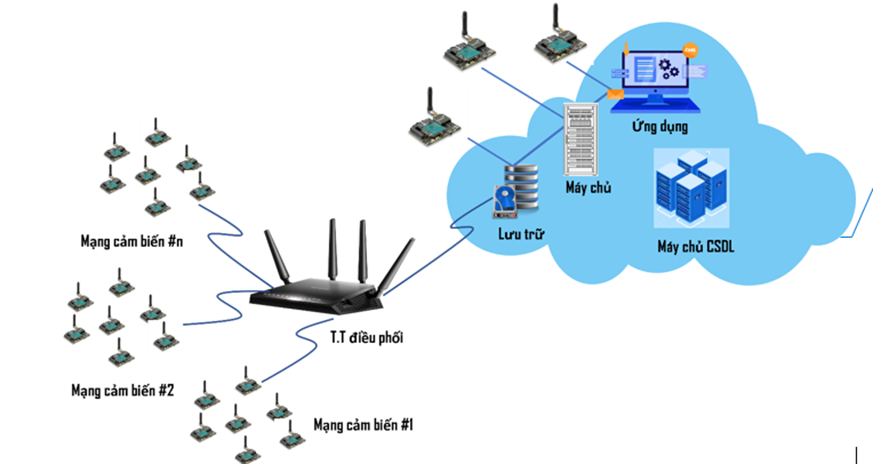
\includegraphics[width=0.8\textwidth]{images/cloud.png}
    \caption{Mô hình tích hợp giữa mạng cảm biến và cấu trúc dữ liệu đám mây}
    \label{cloud}
\end{figure}

Trong hệ thống đề xuất, dữ liệu cảm biến đóng vai trò trung tâm trong việc 
huấn luyện và triển khai các mô hình trí tuệ nhân tạo (AI). Tuy nhiên, bộ nhớ 
của vi điều khiển và thiết bị đầu cuối thường bị giới hạn, do đó giải pháp lưu 
trữ dữ liệu trên nền tảng đám mây là lựa chọn phù hợp và linh hoạt. Việc triển 
khai dữ liệu lên cloud không chỉ giúp loại bỏ rào cản về địa lý, mà còn hỗ 
trợ truy cập, phân tích và chia sẻ dữ liệu từ bất kỳ đâu miễn có kết nối 
Internet. Đồng thời, hệ thống hỗ trợ xuất dữ liệu dưới dạng văn bản (text), 
CSV hoặc JSON, phục vụ nhu cầu chia sẻ giữa các nhóm nghiên cứu.

Về dài hạn, mục tiêu của hệ thống là tích luỹ một tập dữ liệu lớn và đa dạng 
nhằm huấn luyện các mô hình học máy hỗ trợ chẩn đoán và ra quyết định trong 
sàng lọc hội chứng ngưng thở khi ngủ (\gls{OSA}).



\textbf{Cơ sở dữ liệu sử dụng là MongoDB Atlas} với các đặc điểm kỹ thuật nổi bật như sau:
01) Hỗ trợ lưu trữ hiệu quả dữ liệu lớn, phân tán trên nhiều cụm máy chủ, 
cho phép mở rộng theo chiều ngang.
02) Tối ưu hoá truy vấn theo thời gian thực với dữ liệu dạng \texttt{timestamp}.
03) Cơ chế đánh chỉ mục linh hoạt giúp tăng tốc độ truy vấn và giảm dung lượng lưu trữ.
04) Hỗ trợ tự động xoá dữ liệu cũ dựa trên TTL (Time To Live index), 
đồng thời tích hợp trực tiếp với nền tảng MongoDB Atlas.

\begin{figure}[htbp]
\centering
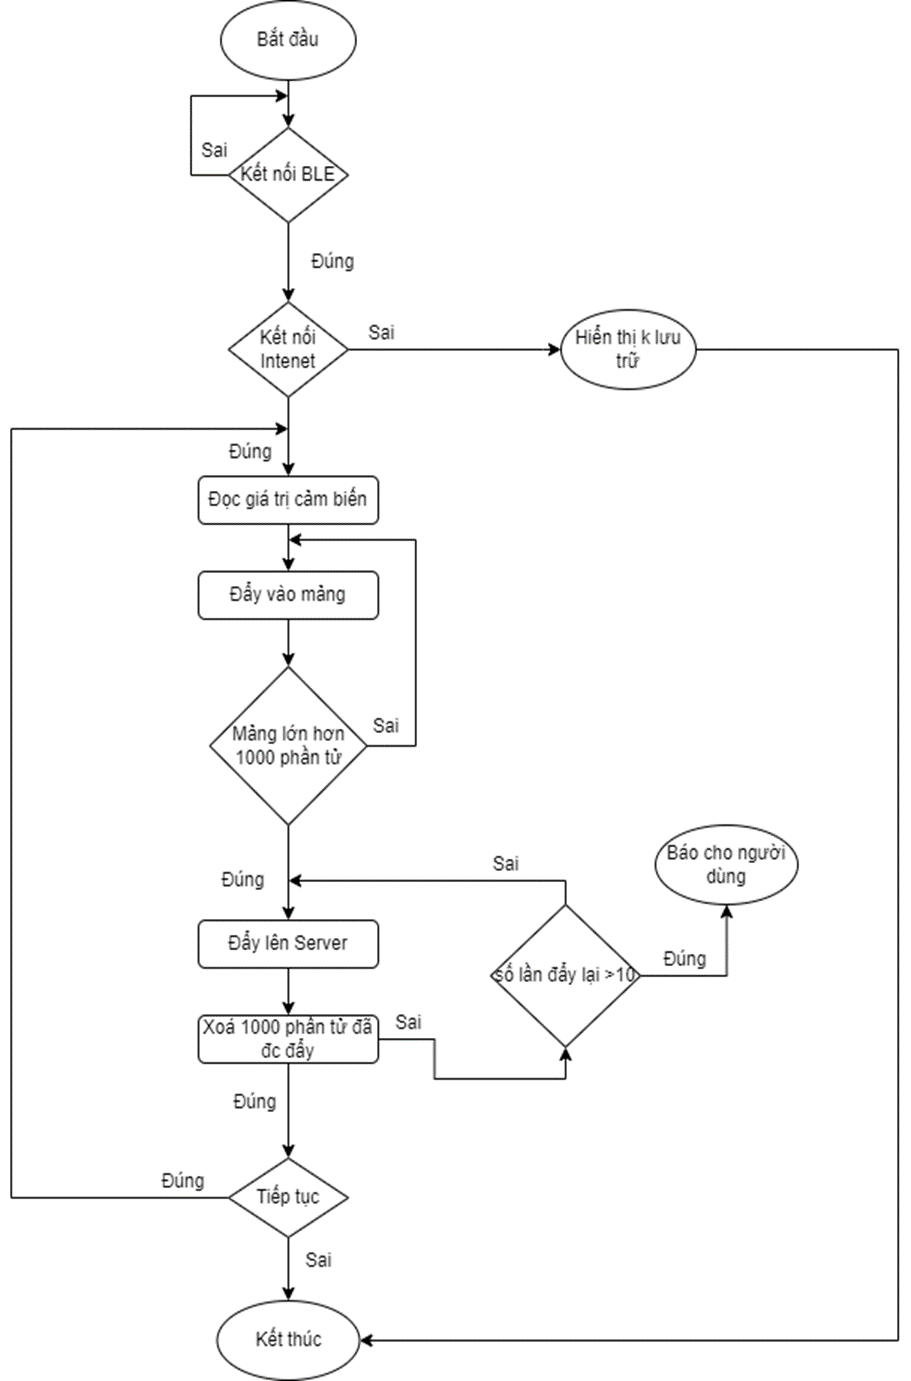
\includegraphics[width=0.9\textwidth]{images/flow_http.png}
\caption{Lưu đồ thuật toán lưu trữ dữ liệu cảm biến}
\label{flow_http}
\end{figure}
Phía máy chủ của hệ thống được xây dựng bằng nền tảng Node.js và triển khai 
trên Amazon Web Services (AWS), cho phép triển khai nhanh, dễ mở rộng và tối 
ưu chi phí trong giai đoạn thử nghiệm. MongoDB Atlas được lựa chọn là hệ quản 
trị cơ sở dữ liệu chính, hỗ trợ gói miễn phí dung lượng 500MB – phù hợp cho 
việc thu thập và đánh giá dữ liệu ở quy mô ban đầu.

Để tránh tình trạng quá tải server khi có nhiều yêu cầu truy cập đồng thời, 
ứng dụng không thực hiện gửi từng mẫu riêng lẻ. Thay vào đó, dữ liệu cảm biến 
sẽ được tích luỹ theo từng lô gồm 1000 mẫu, sau đó mới được gửi lên backend. 
Mỗi mẫu bao gồm ba thành phần gia tốc (\texttt{x, y, z}) và thời gian ghi 
nhận tương ứng, bảo đảm tính toàn vẹn và khả năng truy xuất ngược theo dòng 
thời gian.

Lưu đồ thuật toán lưu trữ dữ liệu được thể hiện trong Hình~\ref{flow_http}, 
gồm hai trường hợp chính:

\vspace{0.5em}
\noindent\textbf{1)} Khi người dùng không có kết nối mạng, hệ thống vẫn cho phép kết nối BLE và hiển thị dữ liệu cảm biến theo thời gian thực, tuy nhiên sẽ không tiến hành lưu trữ lên cloud.

\vspace{0.5em}
\noindent\textbf{2)} Khi người dùng đã đăng nhập và có kết nối Internet, ứng dụng sẽ tự động lưu trữ dữ liệu sau mỗi 1000 mẫu thu thập. Trong trường hợp thao tác gửi dữ liệu thất bại liên tục quá 10 lần, hệ thống sẽ thông báo lỗi và ngừng tiến trình lưu trữ để đảm bảo độ tin cậy.


Ngoài dữ liệu cảm biến thời gian thực được lưu trữ trên MongoDB Atlas, 
hệ thống còn sử dụng cơ sở dữ liệu quan hệ MySQL để quản lý các dữ liệu định 
danh và nghiệp vụ quan trọng khác. Cụ thể:

\vspace{0.5em}
\noindent\textbf{1)} Thông tin người dùng như tài khoản đăng nhập, mật khẩu mã hoá (hash), email, số điện thoại, lịch sử đăng nhập và phân quyền được lưu trữ trong hệ quản trị cơ sở dữ liệu MySQL. Cấu trúc dữ liệu dạng bảng (table) của MySQL giúp đảm bảo tính toàn vẹn quan hệ và dễ dàng thực hiện các truy vấn xác thực người dùng nhanh chóng, an toàn.

\vspace{0.5em}
\noindent\textbf{2)} Các dữ liệu khảo sát lâm sàng như bảng điểm STOP-BANG, thang điểm Epworth, chỉ số BMI, tiền sử bệnh nền và lịch sử đánh giá lặp lại theo từng thời điểm cũng được lưu trong MySQL nhằm đảm bảo tính liên kết logic giữa các thực thể (người dùng – biểu mẫu – kết quả – thời gian).

\vspace{0.5em}
\noindent\textbf{3)} Việc phân chia lưu trữ theo đặc thù dữ liệu (NoSQL cho dữ liệu cảm biến lớn và động, SQL cho dữ liệu người dùng có cấu trúc ổn định) giúp tối ưu hoá hiệu suất truy xuất, tính mở rộng và khả năng bảo trì hệ thống trong dài hạn.

Sự kết hợp giữa MongoDB (dành cho dữ liệu cảm biến, thời gian thực) 
và MySQL (dành cho thông tin người dùng và nghiệp vụ) tạo thành một kiến trúc 
lưu trữ lai (hybrid storage architecture) đáp ứng linh hoạt cả hai loại dữ 
liệu – phi cấu trúc và có cấu trúc – vốn là đặc trưng phổ biến trong các 
hệ thống y tế ứng dụng trí tuệ nhân tạo hiện đại.

\subsection{Học máy trong phân loại tư thế ngủ}

 

\begin{figure}[htbp]
\centering
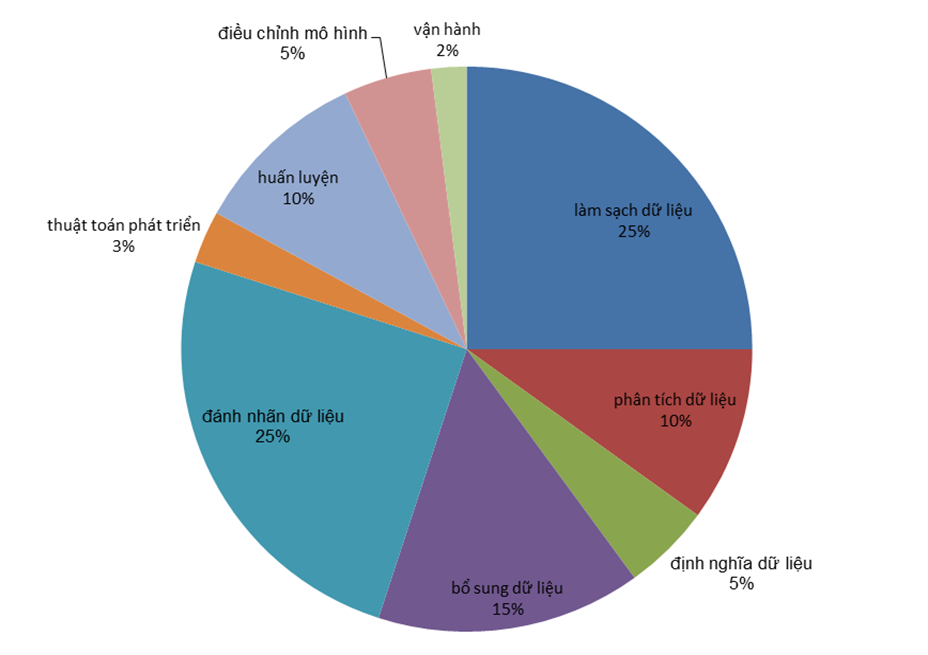
\includegraphics[width=1\textwidth]{images/hocmay_time.png}
\caption{Phân bố thời gian thực hiện đối với dự án học máy}
\label{hocmay_time}
\end{figure}

Hình~\ref{hocmay_time} trình bày phân bố thời gian tương đối giữa các 
công đoạn trong quá trình triển khai một dự án học máy thực tế. 
Dữ liệu trong biểu đồ cho thấy rằng phần lớn thời gian không nằm ở 
bước huấn luyện mô hình, mà được dành cho các công việc tiền xử lý 
dữ liệu – chiếm đến hơn 60\% tổng thời gian.
Cụ thể, hai hoạt động tốn thời gian nhất là \textbf{làm sạch dữ liệu} 
và \textbf{gán nhãn dữ liệu}, mỗi hoạt động chiếm 25\% tổng thời lượng 
thực hiện. Tiếp theo là \textbf{bổ sung dữ liệu} (15\%) và 
\textbf{phân tích dữ liệu} (10\%). Bốn công đoạn này là nền tảng quyết 
định chất lượng đầu vào, ảnh hưởng trực tiếp đến độ chính xác và khả 
năng tổng quát hóa của mô hình sau khi huấn luyện.

Trong khi đó, các bước thường được quan tâm trong các tài liệu học thuật 
như huấn luyện mô hình (10\%), phát triển thuật toán (3\%) và 
tinh chỉnh mô hình (5\%) lại chiếm tỷ trọng thấp hơn. 
Giai đoạn vận hành thực tế (deployment) cũng chỉ chiếm khoảng 2\%, 
tuy nhiên vẫn đóng vai trò quan trọng trong việc chuyển giao ứng dụng 
ra ngoài môi trường thử nghiệm.

Sự phân bố này phản ánh đặc điểm phổ biến trong các dự án học máy với 
dữ liệu thực tế từ cảm biến: chất lượng mô hình phụ thuộc chủ yếu vào 
dữ liệu và quy trình xử lý trước huấn luyện. Do đó, việc đầu tư thời 
gian vào xử lý dữ liệu là hoàn toàn cần thiết và hợp lý.

Tổng quan về các bước xây dựng hệ thống học máy cho bài toán phân loại 
tư thế ngủ đã được trình bày tại Chương~\ref{chapter:1-introduction}.
Trong mục này, tác giả đi sâu vào phân tích các thuật toán học máy 
đã được lựa chọn, lý do lựa chọn, đặc điểm cấu trúc của từng mô hình, 
cũng như hiệu quả của chúng trong bối cảnh bài toán sử dụng dữ liệu 
cảm biến gia tốc ba trục.



\textbf{Hồi quy Logistic (Logistic Regression – LR)} là một trong những thuật toán 
cơ bản và phổ biến nhất trong học máy, đặc biệt phù hợp với các 
bài toán phân loại nhị phân. Về mặt cấu trúc, LR tương tự như hồi 
quy tuyến tính ở chỗ sử dụng tổ hợp tuyến tính giữa các đặc trưng 
đầu vào và trọng số, tuy nhiên kết quả đầu ra được đưa qua một hàm 
kích hoạt phi tuyến gọi là \textbf{hàm logistic (sigmoid)} 
để ánh xạ về miền giá trị $[0, 1]$ \cite{cramer2002logistic}:

\begin{equation}
    \sigma(z) = \frac{1}{1 + e^{-z}}, \quad \text{với } z = \mathbf{w}^T \mathbf{x} + b
\end{equation}

Trong đó, $\mathbf{w}$ là vector trọng số, $\mathbf{x}$ là vector đặc trưng đầu vào, và $b$ là hệ số điều chỉnh (bias). Giá trị $\sigma(z)$ thể hiện xác suất điểm dữ liệu $\mathbf{x}$ thuộc lớp 1. Nếu xác suất này lớn hơn ngưỡng (thường là 0.5), mô hình phân loại $\mathbf{x}$ thuộc lớp dương.

Mặc dù đơn giản và dễ triển khai, hồi quy logistic nguyên thủy chỉ phù hợp với các bài toán phân loại nhị phân. Để mở rộng cho bài toán phân loại đa lớp (multiclass classification), có thể sử dụng biến thể \textbf{Softmax Regression}, trong đó mô hình ước lượng xác suất đầu ra theo phân phối softmax:

\begin{equation}
    P(y = j \mid \mathbf{x}) = \frac{e^{\mathbf{w}_j^T \mathbf{x}}}{\sum_{k=1}^{K} e^{\mathbf{w}_k^T \mathbf{x}}}
\end{equation}

Trong đó, $K$ là tổng số lớp, $\mathbf{w}_j$ là vector trọng số tương ứng với lớp $j$.

Trong khuôn khổ đề tài này, Logistic Regression được lựa chọn nhờ ưu 
điểm về đơn giản, hiệu quả tính toán và kích thước mô hình nhỏ gọn 
(< 5 KB), cho phép triển khai trực tiếp trên các vi điều khiển như 
\texttt{nRF52840}. Mặc dù độ chính xác có thể thấp hơn một số mô hình 
phức tạp hơn như Random Forest hoặc Gradient Boosting, LR vẫn đảm bảo 
hiệu năng chấp nhận được trong bối cảnh hệ thống nhúng giới hạn tài 
nguyên.

\textbf{Máy vector hỗ trợ (Support Vector Machine – SVM)} là một thuật 
toán học có giám sát, đặc biệt hiệu quả cho các bài toán phân loại nhị 
phân với biên ranh giới rõ ràng \cite{cortes1995svm}. Ý tưởng chính của SVM là tìm kiếm một 
\textbf{mặt siêu phẳng (hyperplane)} trong không gian đặc trưng để phân 
chia các điểm dữ liệu thành hai lớp sao cho biên phân cách giữa các lớp 
là lớn nhất.

Trong không gian hai chiều, mặt siêu phẳng tương ứng với một đường thẳng; 
trong không gian ba chiều, đó là một mặt phẳng; và trong không gian 
nhiều chiều hơn, nó là một siêu mặt phẳng tổng quát. 
SVM chọn mặt siêu phẳng sao cho khoảng cách (margin) từ nó đến các 
điểm dữ liệu gần nhất của mỗi lớp – gọi là \textbf{support vectors} – 
là tối đa. Bài toán tối ưu hóa trong SVM có thể biểu diễn như sau:

\begin{equation}
\min_{\mathbf{w}, b} \frac{1}{2} \|\mathbf{w}\|^2 \quad 
\text{subject to } \quad y_i(\mathbf{w}^T \mathbf{x}_i + b) \geq 1, \quad \forall i
\end{equation}

Trong đó, $\mathbf{w}$ là vector trọng số, $b$ là hệ số bias, và $(\mathbf{x}_i, y_i)$ là tập dữ liệu huấn luyện.

Hình~\ref{svm} minh hoạ khái niệm mặt siêu phẳng và các support vectors trong không gian hai chiều.

\begin{figure}[htbp]
    \centering
    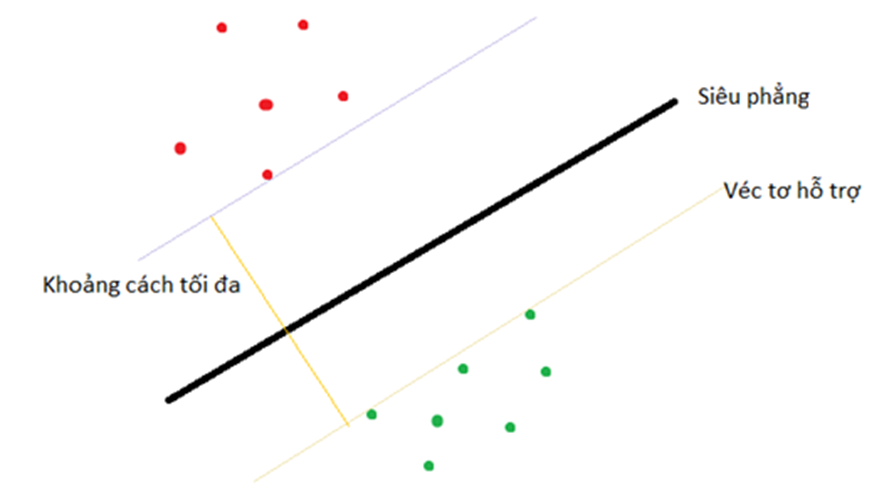
\includegraphics[width=0.6\textwidth]{images/svm.png}
    \caption{Minh họa mặt siêu phẳng phân tách hai lớp trong SVM}
    \label{svm}
\end{figure}
Ưu điểm nổi bật của SVM là khả năng xử lý hiệu quả trong không gian 
đặc trưng cao. Thêm vào đó, SVM có thể mở rộng cho các bài toán 
không tuyến tính thông qua việc sử dụng các hàm kernel, chẳng hạn như 
\textbf{Gaussian RBF kernel} hoặc \textbf{polynomial kernel}, 
giúp ánh xạ dữ liệu vào không gian mới nơi mà việc phân tách tuyến tính 
trở nên khả thi.

Tuy nhiên, SVM cũng tồn tại một số hạn chế. Khi dữ liệu không thể 
phân tách tuyến tính rõ ràng hoặc chứa nhiều nhiễu, hiệu quả phân loại 
có thể suy giảm đáng kể. Ngoài ra, chi phí tính toán trong giai 
đoạn huấn luyện tăng nhanh theo kích thước tập dữ liệu, điều này làm 
cho SVM trở nên khó triển khai trong các hệ thống có tài nguyên hạn 
chế hoặc yêu cầu thời gian thực, như thiết bị nhúng hoặc biên.

Một khái niệm quan trọng trong SVM là \textbf{biên (margin)} – khoảng 
cách giữa mặt siêu phẳng và các điểm dữ liệu gần nhất thuộc hai lớp. 
Mặt siêu phẳng tối ưu là mặt phẳng có biên lớn nhất, và chỉ những điểm 
nằm gần sát biên mới ảnh hưởng đến việc xác định mặt siêu phẳng, 
được gọi là \textbf{các vector hỗ trợ (support vectors)}. Các điểm này 
hỗ trợ việc xác định biên phân cách và trực tiếp ảnh hưởng đến hàm 
quyết định (decision function) của mô hình. Bài toán tối ưu hoá của 
SVM tìm ra các trọng số và bias sao cho biên được cực đại.

Để mở rộng cho các bài toán phân loại đa lớp, có thể áp dụng hai kỹ 
thuật phổ biến: \textbf{one-vs-one} và \textbf{one-vs-rest}, được minh 
hoạ trong Hình~\ref{svm_ovso} và Hình~\ref{ovsr}.

\begin{figure}[htbp]
    \centering
    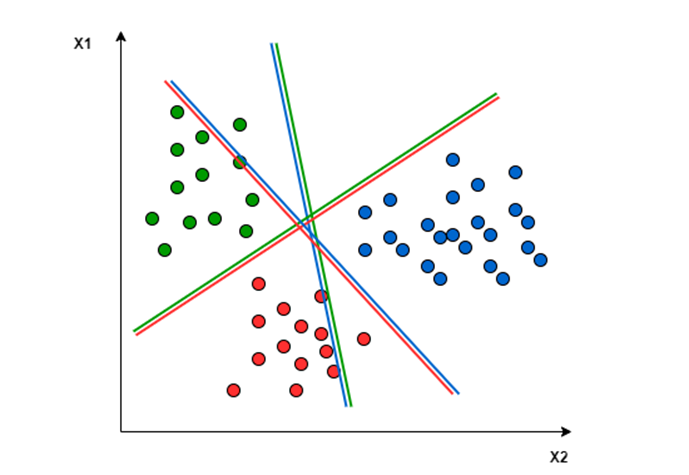
\includegraphics[width=0.6\linewidth]{images/svm_ovso.png}
    \caption{Chiến lược phân loại đa lớp bằng phương pháp One-vs-One}
    \label{svm_ovso}
\end{figure}

\begin{figure}[htbp]
    \centering
    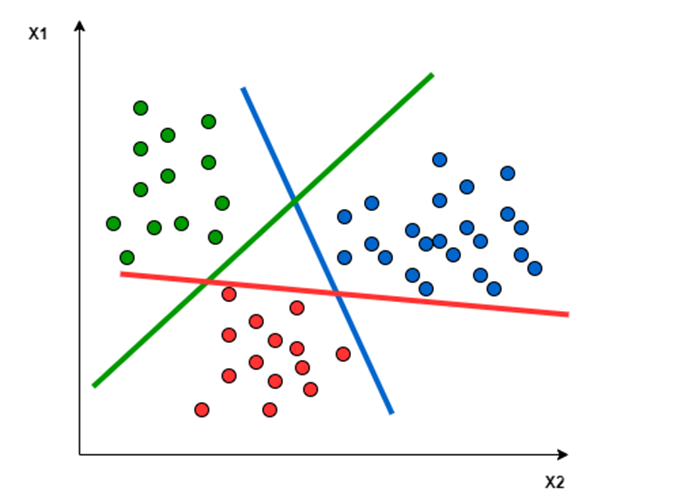
\includegraphics[width=0.6\linewidth]{images/ovsr.png}
    \caption{Chiến lược phân loại đa lớp bằng phương pháp One-vs-Rest}
    \label{ovsr}
\end{figure}

\textbf{One-vs-One (OvO):} Trong phương pháp này, một mô hình SVM được 
huấn luyện cho mỗi cặp lớp. Với $K$ lớp, tổng cộng $\frac{K(K-1)}{2}$ 
mô hình con được huấn luyện. Mỗi mô hình học cách phân biệt giữa hai 
lớp cụ thể và bỏ qua các lớp còn lại. Trong quá trình dự đoán, một cơ 
chế bỏ phiếu (voting) được sử dụng để xác định lớp cuối cùng. 


\textbf{One-vs-Rest (OvR):} Phương pháp này huấn luyện một mô hình cho 
mỗi lớp, trong đó mô hình học cách phân biệt giữa một lớp cụ thể và 
phần còn lại. Với $K$ lớp, ta có $K$ mô hình. Trong quá trình suy luận, 
mô hình đưa ra xác suất hoặc độ tin cậy, và lớp có giá trị cao nhất 
sẽ được chọn.

Cả hai chiến lược OvO và OvR đều giúp mở rộng SVM từ mô hình phân loại 
nhị phân thành phân loại đa lớp hiệu quả, nhưng mỗi phương pháp đều có 
ưu và nhược điểm riêng về thời gian huấn luyện, độ phức tạp tính toán 
và hiệu năng phân loại.



\textbf{Rừng ngẫu nhiên (Random Forest – RF)} là một mô hình học có 
giám sát thuộc nhóm thuật toán tổ hợp (ensemble learning), 
được xây dựng dựa trên nền tảng của 
\textbf{Cây quyết định (Decision Tree)} \cite{breiman2001random}. 
Khác với việc sử dụng một cây duy nhất như trong Decision Tree 
truyền thống, Random Forest xây dựng một tập hợp gồm nhiều cây 
quyết định độc lập, mỗi cây học trên một phần khác nhau của dữ liệu và 
không sử dụng toàn bộ tập thuộc tính. Dự đoán cuối cùng của mô hình 
được xác định thông qua cơ chế biểu quyết (voting) hoặc trung bình hoá 
(trong bài toán hồi quy).

Ý tưởng chính của Random Forest nhằm giảm thiểu hiện tượng 
\textbf{quá khớp (overfitting)} thường gặp trong Decision Tree đơn lẻ. 
Khi xây dựng một cây quyết định mà không giới hạn độ sâu, 
cây có xu hướng học thuộc hoàn toàn dữ liệu huấn luyện, 
dẫn đến khả năng tổng quát kém trên tập kiểm thử. 
RF khắc phục điều này bằng cách đưa vào hai cơ chế ngẫu nhiên chính:

\vspace{0.5em}
\noindent\textbf{1) Lấy mẫu bootstrap:} Mỗi cây được huấn luyện trên 
một tập con của dữ liệu ban đầu, được chọn ngẫu nhiên có lặp lại 
(bootstrap sampling). Như vậy, một phần dữ liệu được bỏ qua, 
làm tăng tính đa dạng giữa các cây.

\vspace{0.5em}
\noindent\textbf{2) Lựa chọn ngẫu nhiên tập thuộc tính:} Tại mỗi nút 
phân chia của cây, chỉ một tập con ngẫu nhiên của các thuộc tính được 
xem xét để chọn điểm chia tốt nhất. Điều này làm giảm sự tương quan 
giữa các cây trong rừng.

Do các cây trong Random Forest được huấn luyện trên những tập dữ liệu 
và tập thuộc tính khác nhau, mỗi cây đơn lẻ có thể có sai số lớn 
(high bias hoặc underfitting). Tuy nhiên, việc tổng hợp kết quả của 
nhiều cây giúp giảm phương sai (variance), cải thiện khả năng tổng 
quát hoá. Nhờ đó, Random Forest đạt được sự cân bằng giữa bias và 
variance – một trong những đặc điểm lý tưởng của mô hình học máy tốt.

Một đặc điểm quan trọng khác là \textbf{tính ổn định} của RF 
đối với nhiễu và dữ liệu không cân bằng, cùng với khả năng 
\textbf{đánh giá mức độ quan trọng của đặc trưng (feature importance)} 
thông qua chỉ số Gini hoặc entropy trung bình trên toàn bộ cây.

Tuy nhiên, mô hình Random Forest có kích thước lớn do lưu trữ nhiều 
cây quyết định, mỗi cây có thể có độ sâu đáng kể. Điều này khiến RF 
khó triển khai trực tiếp trong môi trường hạn chế tài nguyên như các 
vi điều khiển hoặc thiết bị đeo (wearables). Trong nghiên cứu này, 
RF được sử dụng như một mô hình tham chiếu mạnh về độ chính xác, 
nhưng chưa phải là lựa chọn phù hợp cho triển khai biên (TinyML).


\textbf{Học tăng cường (Gradient Boosting – GB)} là một phương pháp học 
có giám sát thuộc nhóm thuật toán tổ hợp (ensemble learning), 
trong đó nhiều mô hình yếu (weak learners) – thường là các cây quyết định có độ sâu nông – 
được kết hợp theo cách tuần tự để tạo thành một mô hình mạnh hơn \cite{chen2016xgboost}.

Khác với Random Forest – nơi các cây được xây dựng song song và độc lập 
– Gradient Boosting xây dựng mô hình theo từng bước lặp (iteration), 
mỗi cây tiếp theo được huấn luyện để sửa lỗi còn lại từ mô hình trước đó. 
Cụ thể, tại mỗi vòng lặp $t$, mô hình hiện tại $F_t(x)$ được cập nhật 
bằng cách cộng thêm một cây mới $h_t(x)$ được huấn luyện để xấp xỉ 
gradient âm của hàm mất mát:

\begin{equation}
F_{t+1}(x) = F_t(x) + \gamma h_t(x)
\end{equation}

Trong đó, $\gamma$ là hệ số học (learning rate), điều chỉnh mức đóng góp của cây mới vào tổng thể mô hình.

Một trong những đặc điểm quan trọng của GB là khả năng 
\textbf{tối ưu hoá trực tiếp một hàm mất mát bất kỳ}, 
chẳng hạn như hàm log-loss trong bài toán phân loại, hoặc hàm bình 
phương sai số (MSE) trong bài toán hồi quy. Nhờ đó, GB thường đạt độ 
chính xác rất cao, đặc biệt trên các bài toán với dữ liệu có quan 
hệ phi tuyến và có nhiều đặc trưng tương tác phức tạp.

Tuy nhiên, Gradient Boosting cũng có những hạn chế rõ rệt. 
Do các cây được xây dựng tuần tự phụ thuộc lẫn nhau, 
GB thường mất nhiều thời gian huấn luyện hơn so với Random Forest. 
Hơn nữa, mô hình nhạy cảm với nhiễu và dữ liệu nhiễu sẽ dễ dàng 
bị mô hình "học theo", dẫn đến hiện tượng quá khớp (overfitting) 
nếu không áp dụng kỹ thuật regularization hoặc early stopping.

Trong nghiên cứu này, tác giả sử 
dụng \textbf{GB} để phân loại tư thế ngủ đạt độ chính xác cao nhất, điều này đúng trên toàn bộ kịch bản thử nghiệm.
Tuy nhiên, do số lượng cây lớn và trọng số tổng thể cao (trên 500~KB), Gradient Boosting chưa phù hợp để triển khai 
trực tiếp trên các thiết bị vi điều khiển hạn chế tài nguyên. Thay vào đó, mô hình này được sử dụng để thiết lập ngưỡng hiệu năng tham chiếu (baseline) trong môi trường huấn luyện trên máy chủ hoặc máy tính cá nhân.


\textbf{Mạng nơ-ron nhân tạo (Artificial Neural Network – ANN)} là một 
mô hình học sâu mô phỏng cấu trúc hoạt động của hệ thần kinh sinh học, 
trong đó các nơ-ron nhân tạo (artificial neurons) được tổ chức thành nhiều 
lớp (layers) và kết nối với nhau qua các trọng số (weights) \cite{jain1996}. 
Trong nghiên cứu này, tác giả sử dụng kiến trúc \textbf{Multilayer Perceptron (MLP)} – 
một loại mạng nơ-ron đơn giản gồm ít nhất ba lớp: lớp đầu vào (input layer), 
một hoặc nhiều lớp ẩn (hidden layers) và lớp đầu ra (output layer).

Mỗi nơ-ron trong lớp ẩn thực hiện một tổ hợp tuyến tính giữa các đầu vào, 
sau đó áp dụng một hàm kích hoạt phi tuyến như hàm ReLU 
(Rectified Linear Unit):

\begin{equation}
    f(x) = \max(0, x)
\end{equation}

Đầu ra của mạng được tính thông qua lan truyền tiến (forward propagation), 
và mô hình được huấn luyện bằng cách tối thiểu hóa một hàm mất mát 
(loss function), chẳng hạn như hàm binary cross-entropy trong phân 
loại nhị phân, thông qua thuật toán lan truyền ngược (backpropagation) và 
phương pháp tối ưu như \texttt{Adam} hoặc \texttt{SGD}.

Ưu điểm chính của mạng nơ-ron là khả năng học các quan hệ phi tuyến 
phức tạp và tự động trích xuất đặc trưng từ dữ liệu. Khác với các mô 
hình tuyến tính như LR hoặc SVM, ANN có thể biểu diễn các ranh giới 
phân lớp không tuyến tính và phù hợp với các bài toán tín hiệu cảm 
biến có nhiễu, biến đổi theo thời gian hoặc không gian.

Tuy nhiên, ANN cũng tồn tại nhiều thách thức trong thực tế triển khai:
01) Lựa chọn tham số
02) Yêu cầu tính toán cao
03) Khó giải thích: ANN hoạt động như một hộp đen, 
khó hiểu về mặt trực quan so với cây quyết định hoặc hồi quy logistic.

Trong đề tài này, tác giả sử dụng một kiến trúc MLP đơn giản gồm hai lớp ẩn với 
số lượng nơ-ron tương đối nhỏ $(8, 4)$ và hàm kích hoạt ReLU, 
được huấn luyện bằng thuật toán tối ưu \texttt{Adam} với 
tốc độ học ban đầu là $0.01$.


\textbf{Convolutional Neural Network (CNN)} là một mô hình học sâu được 
thiết kế chuyên biệt để xử lý các loại dữ liệu có cấu trúc lưới, 
chẳng hạn như ảnh hai chiều hoặc tín hiệu chuỗi thời gian một chiều. 
Không giống như mạng neural truyền thống, CNN sử dụng phép tích chập 
để trích xuất tự động các đặc trưng cục bộ trong dữ liệu, từ đó giảm 
thiểu đáng kể nhu cầu tiền xử lý và cải thiện hiệu quả học biểu diễn 
\cite{lecun2015deep}.


Một kiến trúc CNN điển hình bao gồm các tầng tích chập 
(convolutional layers), tiếp theo là các hàm kích hoạt phi tuyến như 
ReLU và các tầng giảm mẫu (pooling layers). Sau các tầng này, các 
đặc trưng được đưa vào một hoặc nhiều tầng kết nối đầy đủ 
(fully connected layers) để thực hiện phân loại. 
Quá trình này cho phép CNN học được cả đặc trưng cục bộ lẫn 
toàn cục trong tín hiệu đầu vào.

Tuy nhiên, trong khuôn khổ của nghiên cứu này, mục tiêu chính không chỉ 
là đạt độ chính xác tối đa mà còn là đánh giá ảnh hưởng của các 
đặc trưng (features) trên miền thời gian và miền tần số đối với 
hiệu suất của mô hình học máy nên tác giả quyết định chọn LR, SVM, RF, GB, NN để tiến hành thử nghiệm. 
Để thực hiện điều đó, tác giả xây dựng 
tám kịch bản khác nhau tương ứng với các tổ hợp đặc trưng và 
kích thước cửa sổ khác nhau. Việc huấn luyện và đánh giá trên nhiều 
kịch bản đòi hỏi một mô hình đủ linh hoạt, dễ kiểm soát về kích thước 
và thời gian huấn luyện.




